\documentclass[10pt]{scrartcl}
\usepackage[english]{babel}
\usepackage{multirow}
\usepackage[default]{opensans}
\usepackage{sfmath} % sans font also for math
\usepackage[binary-units = true]{siunitx}
\usepackage{graphicx}
% defining the paper layout that no text overlaps with the header
\usepackage[
  top=35mm,
  headheight=25mm,
  headsep=3mm,
  bottom=30mm,
  left=25mm,
  right=25mm
]{geometry}

\usepackage[verbose]{placeins}
\usepackage{subcaption}
\usepackage{latexsym}
\usepackage[centertags]{amsmath}
\usepackage{amssymb}
\usepackage[]{glossaries}

\graphicspath{{figures/}}
% custom header and footpage
\usepackage{scrpage2}
\pagestyle{scrheadings} % you have to set the custom layout
% Head
%\chead{}
\ohead{
\includegraphics[height=25mm]{figures/EUCALL.png}}
% Foot
\ifoot{
\includegraphics[height=13.4mm]{figures/EU.png}} % left foot
\cfoot{%
  \begin{minipage}{100mm}%
    \begin{scriptsize}%
      \normalfont{This project has received funding from the}
      \textit{European Union’s Horizon 2020 research and innovation programme}
      \normalfont{under grant agreement No 654220.}
    \end{scriptsize}%
  \end{minipage}%
} % center foot
\ofoot{\thepage} % right foot

\usepackage{booktabs}

%%%%%%%%%%%%%%%%%%%%%%%%%%%%%%%%%%%%%%%%%%%%%%%
%   BIBLIOGRAPHY SETTINGS
\usepackage[bibstyle=nature,sorting=none,maxnames=1000,eprint=false,
defernumbers=true, backend=biber]{biblatex}
\usepackage{chemformula}
\usepackage{hyperref}


\renewcommand*\finalnamedelim{, and\addspace}
\DeclareNameAlias{sortname}{last-first}
\renewcommand{\newunitpunct}{, }

\AtEveryBibitem{%
  \clearfield{day}%
  \clearfield{month}%
  \clearfield{endday}%
  \clearfield{endmonth}%
  \clearfield{issn}%
  \clearfield{issue}%
}
%convert titles to hyperlinks using doi
\ExecuteBibliographyOptions{doi=true} \newbibmacro{string+doi}[1]{%
  \iffieldundef{doi}{#1}{\href{http://dx.doi.org/\thefield{doi}}{#1}}}
  \DeclareFieldFormat*{title}{\usebibmacro{string+doi}{\mkbibemph{#1}}}

\addbibresource{urls.bib}
\addbibresource{footnotes.bib}
\addbibresource{library.bib}

%%%%%%%%%%%%%%%%%%%%%%%%%%%%%%%%%%%%%%%%%%%%%%%
% GLOSSARY SETTINGS
\setacronymstyle{long-short}
\input{glossary}
\makeglossaries
%%%%%%%%%%%%%%%%%%%%%%%%%%%%%%%%%%%%%%%%%%%%%%%

% Zeilenabstand
\renewcommand{\baselinestretch}{1.2}

\usepackage[final]{pdfpages}
\usepackage{pgfplots}
\usepackage{tikz}
\usetikzlibrary{automata,shapes,snakes,positioning}
\usepackage{mathtools}
\DeclarePairedDelimiter\ceil{\lceil}{\rceil}
\DeclarePairedDelimiter\floor{\lfloor}{\rfloor}


\ihead{D4.5} % left head

% sophisticated linking of references in the pdf and setting some options
\usepackage{url}                                                  % for correct typesettings of URLs
\usepackage{hyperref}                                             % for sophisticated linking of urls, dois, pictures, tables, etc.
\hypersetup{
    unicode=true,                                                 % non-Latin characters in Acrobat’s bookmarks
    pdftoolbar=true,                                              % show Acrobat’s toolbar?
    pdfmenubar=true,                                              % show Acrobat’s menu?
    pdffitwindow=false,                                           % window fit to page when opened
    pdfstartview={FitH},                                          % fits the width of the page to the window
    pdftitle={D4.5: Testing, validation, and example workflow},   % title
    pdfauthor={C. Fortmann-Grote},                                % author
    pdfsubject={EUCALL WP4 (SIMEX) Deliverable D4.5},             % subject of the document
    pdfcreator={pdflatex},                                        % creator of the document
    pdfnewwindow=true,                                            % links in new PDF window
    colorlinks=true,                                              % false: boxed links; true: colored links
    linkcolor=blue,                                               % color of internal links (change box color with linkbordercolor)
    citecolor=blue,                                               % color of links to bibliography
    filecolor=blue,                                               % color of file links
    urlcolor=blue                                                 % color of external links
}

% Zeilenabstand
\renewcommand{\baselinestretch}{1.2}

\begin{document}
\makeatletter
\begin{titlepage}
\thispagestyle{scrheadings}
\begin{center}
$~$\\
\vspace{0cm}
{\Large\textbf{EUCALL}\\[2ex]
The European Cluster of Advanced Laser Light Sources}\\[4ex]
%
{\small\textbf{Grant Agreement number: 654220}}\\[6ex]
%
Work Package 4 -- SIMEX\\[3ex]
%
Deliverable D4.5\\
%
Testing, validation, and example workflow\\[4ex]
%
Lead Beneficiary: DESY\\[4ex]
%
Carsten Fortmann-Grote,
Johannes Reppin,
Frank Schl\"unzen,
Yves Kempp,
Sergey Yakubov,
Ashutosh Sharma,
Alexander Andreev,
Sakura Pascarelli,
Mathias Sander,
Thomas Kluge,
Marco Garten,
Axel H\"ubl,
Michael Bussmann,
and
Adrian P. Mancuso\\[4ex]
%
Due date: September 30, 2018\\
Delivery date: \today \\[4ex]
%
Project webpage: \url{www.eucall.eu}\\[6ex]
%
{%
\small
\begin{tabular}{|l|l|}
  \hline
  \multicolumn{2}{|l|}{ \textit{Deliverable Type} } \\
  \hline
  R = Report\hfill & R\\
  DEM = Demonstrator, pilot, prototype, plan designs & \\
  DEC = Websites, patents filing, press \& media actions, videos, etc. & \\
  OTHER = Software, technical diagram, etc. & \\
  \hline
  \multicolumn{2}{|l|}{\textit{Dissemination level}} \\
  \hline
  PU = Public, fully open, e.g. web & PU \\
  CO = Confidential, restricted under conditions set out in Model Grant
  Agreement\hspace*{17ex}\  & \\
  CI = Classified, information as referred to in Commission Decision 2001/844/EC
  & \\
  \hline
\end{tabular}
}

\end{center}
%
%\vfill
\centering{%

\includegraphics[width=0.91\textwidth]{figures/PartnerLogos_2017}
}
\normalfont
\end{titlepage}
\makeatother

\section*{Abstract}
%
This report details validation and benchmark studies of the experiment simulation capabilities
developed in EUCALL's workpackage 4 (SIMEX). Where available, we compare our
simulations to experimental data. In other cases, we compare simulations with
simulations, using either different implementations of the same modeling
approach or two simulations of varying degree of accuracy (e.g. 1D vs. 2D
radiation hydrodynamics). The second part contains HPC benchmarks of selected
simulation codes which present performance bottlenecks in the respective
simulation pipeline.
%
\tableofcontents
%
\section{Validation}%
\subsection{Single--particle coherent diffractive imaging\label{sec:single_particle_imaging}}
We present two study cases where we validate and benchmark individual simulation
modules as well as an entire start--to--end simulation toolchain with
experimental data. In the first case, we compare simulated and measured 2D
diffraction data from the Rice Dwarf Virus \cite{Munke2016}, in the second case
we compare 3D molecular structures reconstructed from simulated diffraction data
to the original 3D model reconstructed from NMR \cite{Schlessman1998}
measurements.
\subsubsection{Validation of single--particle imaging using measured diffraction data }
Our validation of the single--particle imaging simulation toolchain in SIMEX
uses diffraction data measured at the AMO endstation at
\SI{1.6}{\kilo\electronvolt} photon energy.
%
\begin{verbatim}
TBC (Carsten)
\end{verbatim}
%
\subsubsection{Validation of the single--particle imaging simulation toolchain
using reconstructed density profiles}%
%
\begin{figure}[ht]
  \begin{center}
    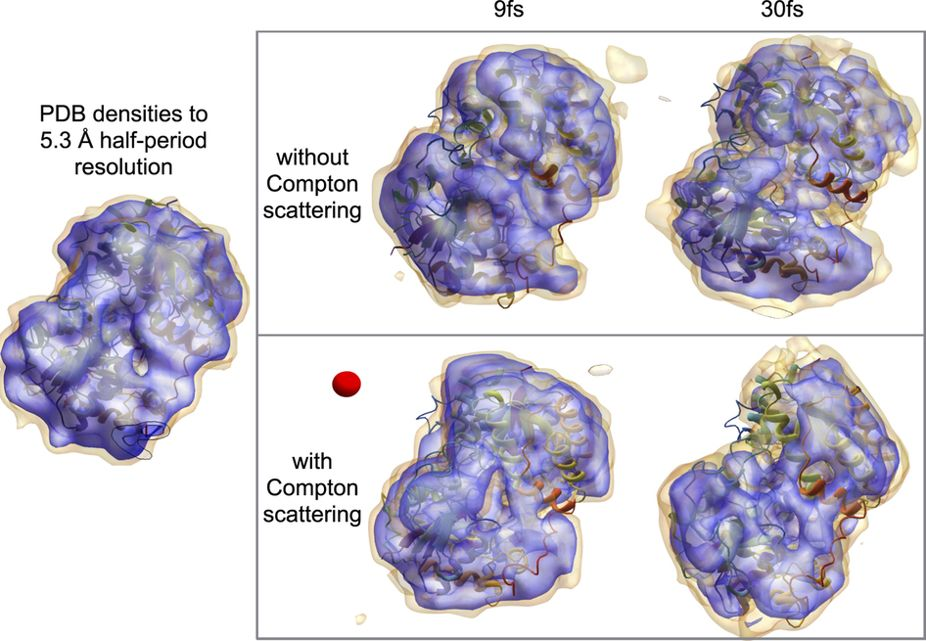
\includegraphics[width=0.8\textwidth,angle=0,clip]{srep24791-f7}
  \end{center}
  \caption{Electron densities of the average reconstruction at the 5\% and 15\%
    levels (yellow and purple, respectively) from simulated diffraction data with
    (top row) and without (bottom row) Compton scattering and for two different
    XFEL pulse durations. The protein's low--resolution features (original PDB
    shown on left-hand-side) were recovered in
    all four cases, with surface electron densities showing the most variation and
    hence least certainty. Loss of reproducible density is more severe in the
    30 fs case due to greater damage. Degradation of surface contrast is
    expected in
    previous damage--only simulations and may, in future studies, be tampered by a
    sacrificial water layer\cite{Hau-Riege2004}. Reproduced
    from Yoon et al., Scientific Reports \textbf{6}, 24791 (2016) under the
    Creative Commons Attribution 4.0 International License.
  }
  \label{fig:2NIP_reconstruction}
\end{figure}

Coherent diffraction from single proteins has been simulated using the
\textit{simS2E} suite \cite{Yoon2016}. Of the order 200000 diffraction images,
sampling the FEL spectral and temporal fluctuations, including focussing
mirror height profiles, radiation damage processes (ionization and atomic
displacement), were then fed into computational reconstruction using the
Expand--Maximize--Compress (EMC) algorithm for orientation and the
Difference Map (DM) algorithm to solve the phase problem. The resulting 3D
electron density maps could then be compared to the PDB model that was used as
a sample specification in the simulation. The structure in the PDB had been
measured with the NMR method. We reproduce in Fig.~\ref{fig:2NIP_reconstruction}
the corresponding results from the original article by Yoon et al.
The results demonstrate the predictive power of our start--to--end simulation
toolchain. All main features of the protein were reproduced. Regions close to
the surface show enhanced displacement and poorer agreement with the
experimental data due to radiation damage.
%
\subsection{Coherent Nanocrystal diffraction\label{sec:coherent_nanocrystal_diffraction}}
Two codes integrated in \textit{simex\_platform} can be used to model x--ray
diffraction from crystalline samples. The first code is \textit{singfel},
which calculates the diffraction from given atomic coordinates and scattering
formfactors. The second code is \textit{pattern\_sim} (part of
\textit{crystfel}) \cite{White2012}, which
reads only the crystallographic unit cell and form factors plus information
about the point group and sample size to calculate the diffraction
pattern consisting of Bragg spots and incoherent contributions.
\textit{singfel} reads the structure of the entire nanocrystal, thus providing
more flexibility to account for radiation damage effects which break the
translational symmetry of the sample.
%
\begin{figure}[ht]
  \begin{center}
      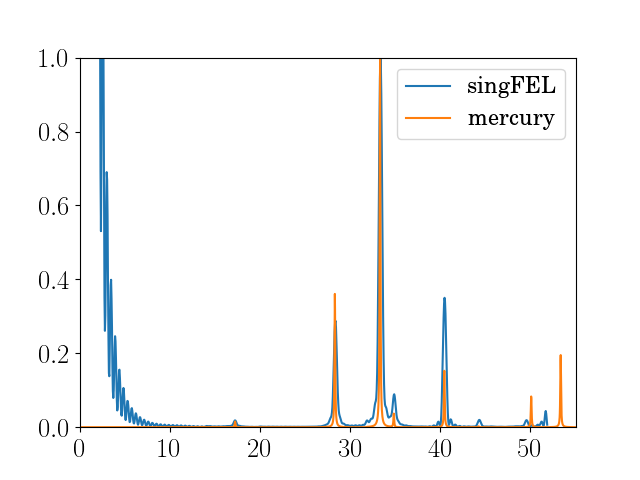
\includegraphics[width=.49\textwidth,angle=0,clip]{Fe2O3_vpp_mercury_vs_simex}
      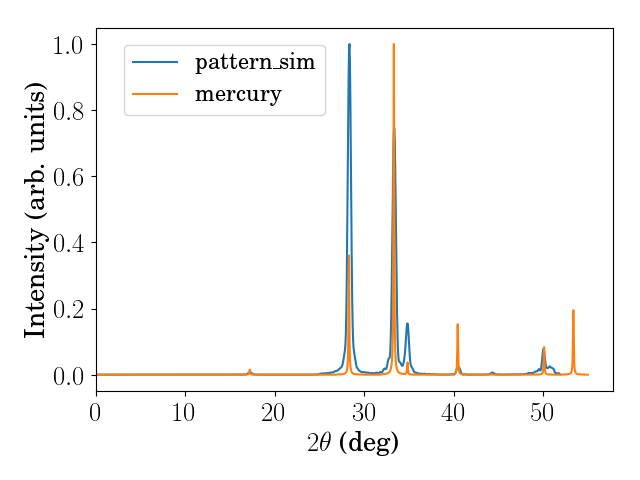
\includegraphics[width=.49\textwidth,angle=0,clip]{Fe2O3_vpp_mercury_vs_patternsim}
  \caption{Simulated powder diffraction patterns (blue lines) for nanocrystalline fcc Fe\textsubscript{2}O\textsubscript{3}
  using the diffraction modules \textit{singfel} (left) and \textit{pattern\_sim}
  (right) compared to reference calculations for an infinite fcc lattice
    using the code \textit{mercury} (orange curve).}
    \label{fig:Fe2O3_vpp_model_vs_model}
  \end{center}
\end{figure}
%
We validate both codes against the code \textit{mercury} \cite{Macrae2008} of the
Cambridge Crystallographic Data Centre (CCDC). Fig.~\ref{fig:Fe2O3_vpp_model_vs_model} shows the simulated
powder diffraction pattern up for \textit{singFEL} vs. \textit{mercury} (left)
and for \textit{pattern\_sim} vs. \textit{mercury} (right). The sample is a
\SI{18}{\nano\metre} sized fcc crystal of
Fe\textsubscript{2}O\textsubscript{3}. In both cases, the
positions of Bragg peaks produced by SIMEX correspond to the reference
simulation. In general, the peak amplitudes differ between the SIMEX simulations and the
reference model, while the \textit{singFEL} results are in better agreement to the
reference model than the \textit{pattern\_sim} results. This difference between
\textit{singFEL} and \textit{pattern\_sim} can be attributed to the more
precise and well validated model for the form factors, calculated with the code \textit{XATOM}
\cite{Son2011}. Note that the \textit{singFEL} calculation contains a
large signal at small angles, this has been removed in the \textit{pattern\_sim}
calculation. These simulations were used to support the feasibility of a
experiment proposed at European XFEL.

In the following, we will
apply the \textit{singFEL} module for diffraction simulations and compare to
experimental data.
Fig.~\ref{fig:C60_virtual_powder_data_vs_models} compares \textit{singfel}
simulations to diffraction data from
an experiment at the CXI endstation at LCLS in a virtual powder representation.
The sample is fcc nanocrystalline C\textsubscript{60}. Bragg peaks were identified in each measured
2D diffraction pattern using the \textit{psana} \cite{psana_www} peak finder
and histogrammed according to the peak's
radial distance from the geometrical center of the detector image corresponding
to zero scattering angle.
The histogram (orange bars) is plotted as a function of the Bragg
angle $2\theta$ and compared to a SIMEX simulation using \textit{singfel}
(blue curve) and the \textit{mercury} reference calculation for a perfect
infinite fcc lattice. Similar to the model--vs--model comparison, the agreement
between models and data is overall satisfying, i.e. the peak positions coincide
and the peak amplitudes are close.
%
\begin{figure}[ht]
  \begin{center}
    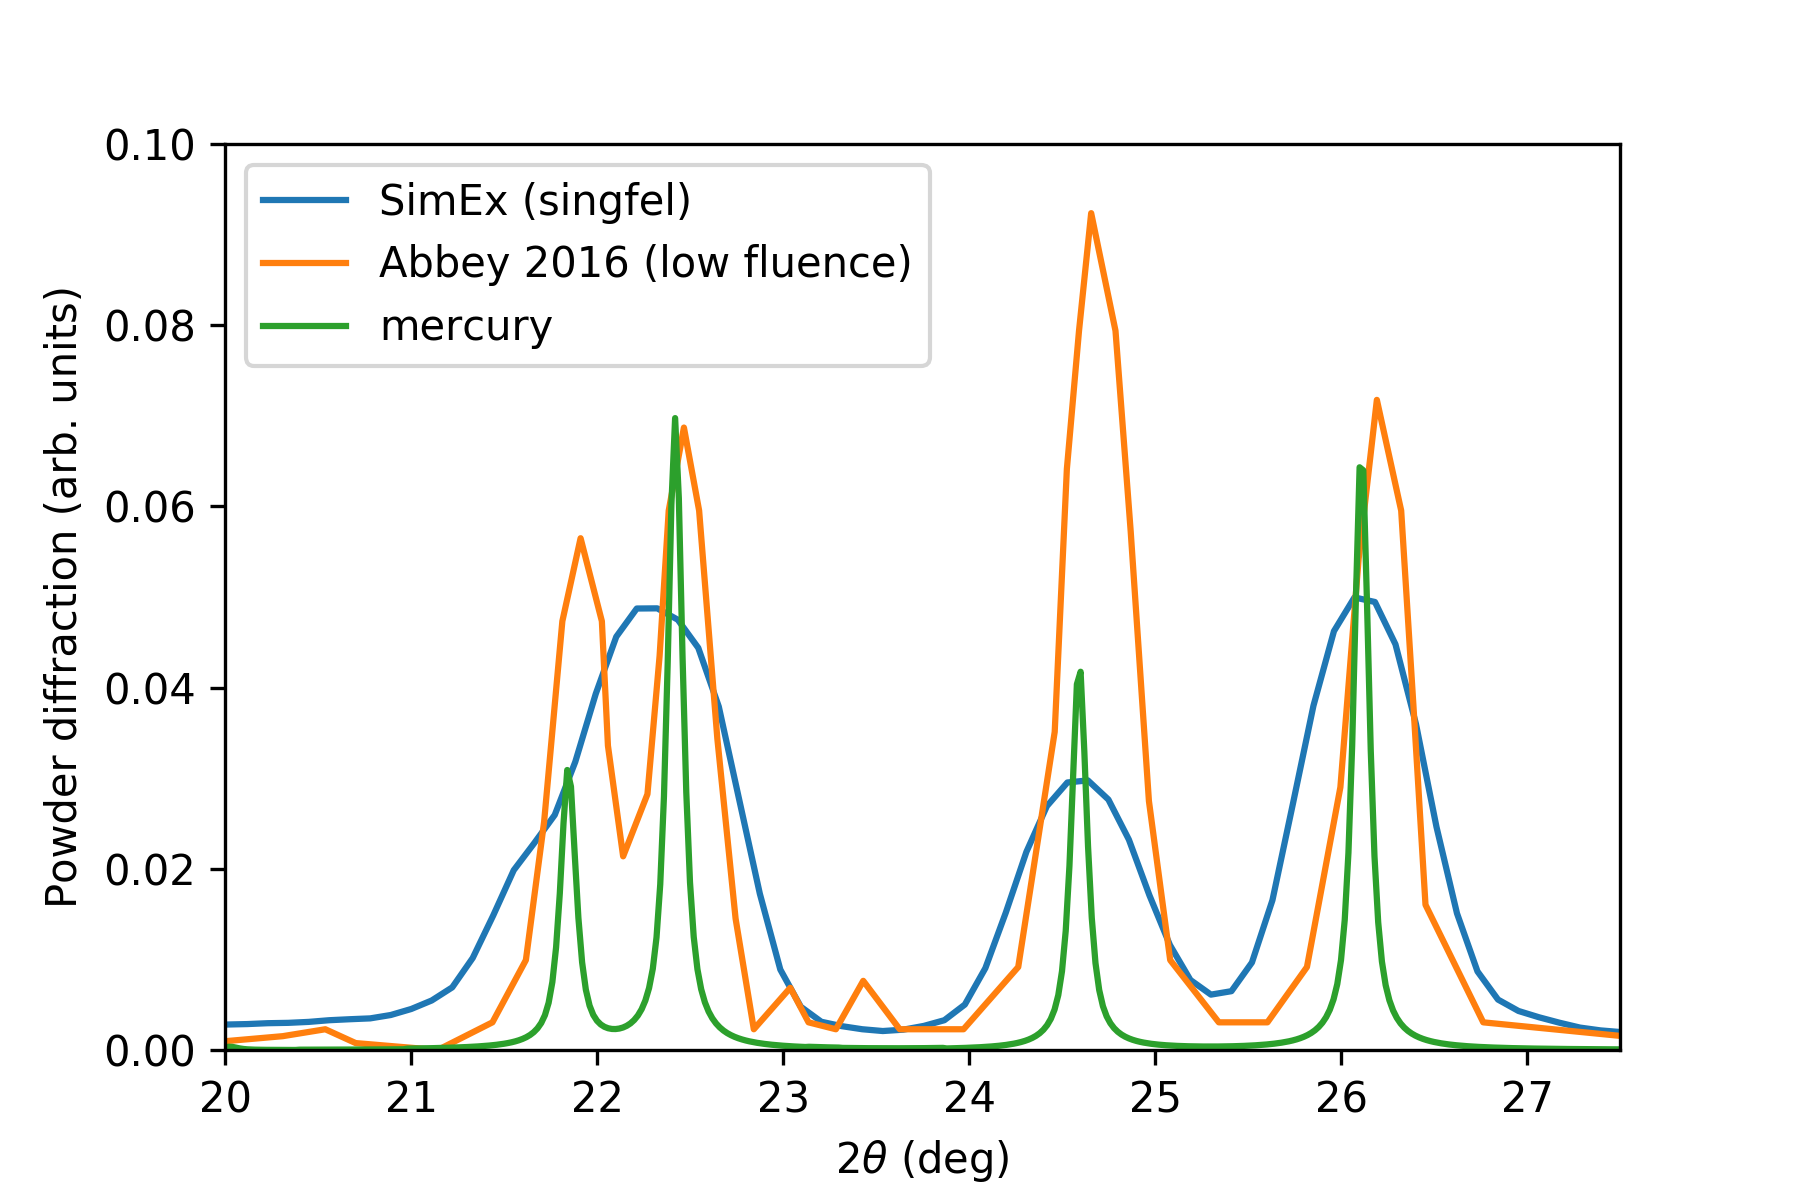
\includegraphics[width=.8\textwidth,angle=0,clip]{C60_Abbey2016_phaseAfcc_lowFluence_vs_simex_noRD}
    \caption{Virtual powder pattern from nanocrystalline C\textsubscript{60}
    \cite{Abbey2016} (orange curve) compared to SIMEX
    simulations for a 10x10x10 C\textsubscript{60} fcc supercell using the code
    \textit{pysingfel} (blue curve) and compared to a modeled powder pattern for
    an infinite C\textsubscript{60} fcc lattice using the code \textit{mercury}.}
    \label{fig:C60_virtual_powder_data_vs_models}
  \end{center}
\end{figure}
%
\subsection{Imaging of High--Power Laser driven targets\label{sec:high_power_imaging}}
In Deliverable Report D4.3 \cite{Fortmann-Grote2017e}, we presented the interoperability
of X-ray Free-Electron Laser (XFEL) and Ultra-High Intensity (UHI) laser pulse
generation, interaction with the target, and generation of a Small-Angle X-ray
Scattering (SAXS) images using the scattering code ParaTAXIS.  A Particle In
Cell (PIC) simulation provides the time evolution of the electron density on
which the XFEL photons are scattered.  We assumed invariance of the target in
propagation direction and simulated the XFEL pulse with $10^{12}$ photons for
which the target is optically thin.  The ion density follows the electron
density as expected for plasma expansion into vacuum.  The SAXS pattern well
resolves the nanometer-scale grating depth and period, taking into account the
target evolution during the interaction time with the laser pulse.  The full
details were reported in Deliverable4.3 \cite{Fortmann-Grote2017e} and
Deliverable D4.4 \cite{Fortmann-Grote2017h}. The simulation
parameters match an experiment led by the group of HZDR which was recently
published in \cite{Kluge2017}.  In the experiment a silicon grating was irradiated by a
Ti:Sa laser with $400$\,mJ on target and pulse duration $80$\,fs, focus size
$1500\,\mathrm{\mu m^2}$ (FWHM).  The expansion of the grating as a function of
time was measured and is reported in [!!1].
%
\begin{figure}
  \begin{center}
    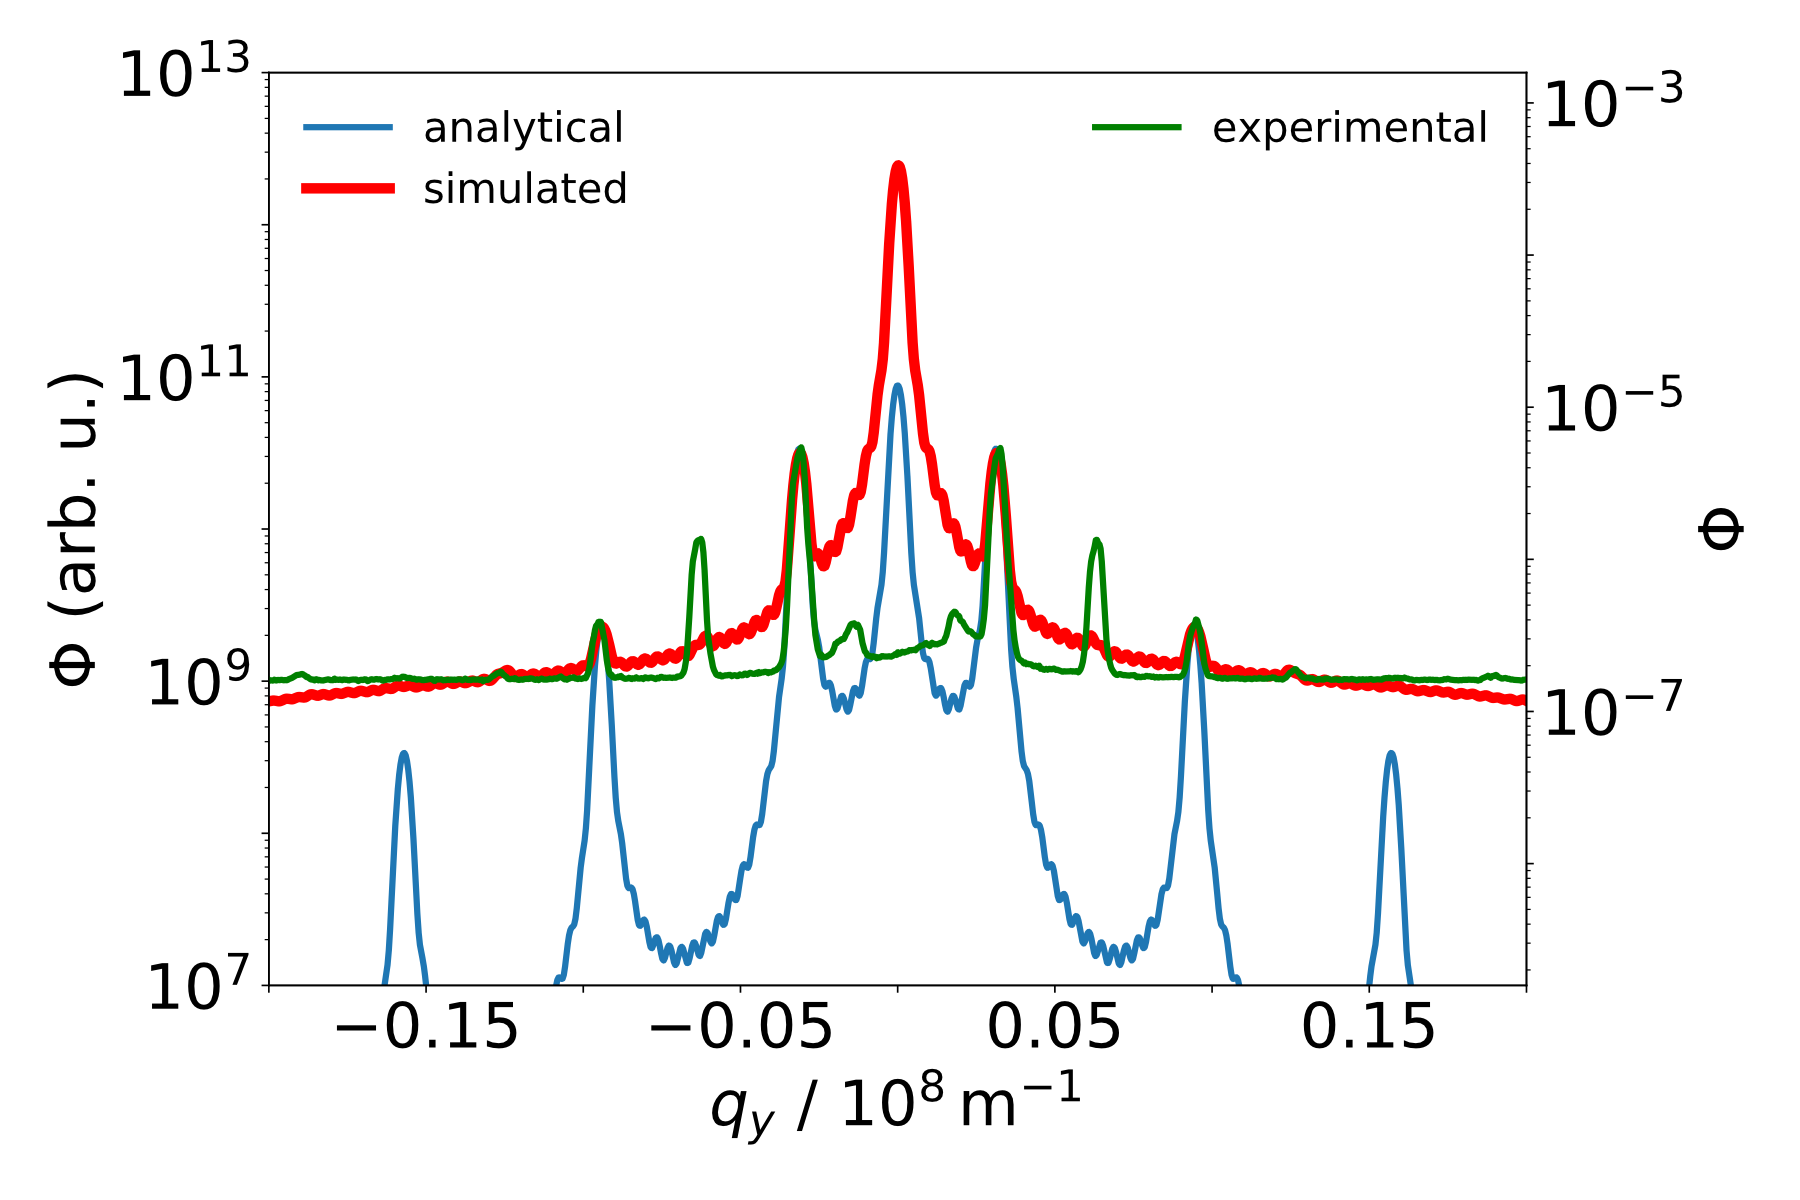
\includegraphics[width=0.8\textwidth]{figures/parataxis_vs_ln04.png}
    \caption{Comparison between the ParaTAXIS simulated scattering profile
      (red)
      and the analytic solution (blue), both based on PIC-simulated data
      used
      also in [Kluge et al. ``Observation of ultrafast solid-density
        plasma
        dynamics using femtosecond X-ray pulses from a free-electron
        laser'',
      arXiv:1801.08404].
      The two curves almost perfectly agree in the relative
      heights of the scattered peaks, the signal in between is
      larger in the ParaTAXIS simulation due to the finite number of
      quasi-photons in the simulation.
      The simulation also agrees reasonably well with the
      experimental data, taking into account the finite experimental
      background  and imperfect peak-to-valley aspect ratio of the front
      side grating, generating imperfect suppression of even scattering
      peaks.
    }\label{fig:parataxis_vs_ln04}
  \end{center}
\end{figure}
%
Here we compare the scattering patterns at $t=0$ (i.e. when the laser maximum
has reached the target front surface) between the ParaTAXIS simulation, an
analytic solution and the measurement (see Fig.~\ref{fig:parataxis_vs_ln04}).
For optically
thin targets, the scattering pattern of a grating with soft edges can be
described by an analytic equation (\cite{Kluge2018}). As an input into this equation
we extract the sharpness of the grating edges from the simulation,
$\sigma\approx 8 nm$ We find a good agreement between the simulation and the
analytic solution, as well as with the experimental curve when we take into
account a few key aspects.  First, we note that the ParaTAXIS simulation gives
the same relative peak heights as the Fourier transform, validating the
simulation.  The signal level between the main peaks is different however due to
the finite number of quasi-photons used in the simulation.  With more simulation
time, this level will further decrease, as this contribution is solely due to
limited sampling of the full parameter space for the quasi-photons and will be
fully extinct in the limit of high photon numbers.  Secondly, the experiment
contains signal from a background contribution, e.g. from plasma self-emission,
bremsstrahlung and 3rd harmonic of the drive laser.  Also, the experiment shows
peaks in between the simulated peak positions, which are due to non-perfect
aspect ratio of the pre-inscribed grating on the target surface.  In the
simulated case, the initial peak-to-valley aspect ratio is 1:1, while in the
experiment due to production uncertainties this is not exactly the case.
Besides this difference the experimental results are reproduced well by the
simulation.

%
\subsection{Liquid jet crystal diffraction\label{sec:liquid_crystals}}
\begin{verbatim} TODO: Mathias (ESRF) \end{verbatim}

\subsection{Warm dense matter x--ray absorption spectroscopy\label{sec:warm_dense_matter_spectroscopy}}
Interaction of high--energy optical laser pulses with solid targets and shock
compression is modeled with radiation--hydrodynamics (RH) simulations using
either 1D (\textit{Esther} \cite{Colombier2005})
or 2D (\textit{Multi2D} \cite{Ramis2009}) RH implementations.
The resulting profiles for mass density, temperature,
ionization, and pressure are then fed into an electronic structure calculation.
Finally, a real--space Green function code (e.g. FEFF \cite{Rehr2009} calculates the x--ray absorption
spectrum. At this point, the spectrum and intensity distribution of the x--ray
probe beam, delivered by x--ray raytracing simulations can be taken into
account. The workflow, supported by SIMEX is shown in
Fig.~\ref{fig:xas_workflow}.
%
\begin{figure}[ht]
  \begin{center}
    \includegraphics[width=0.8\textwidth,angle=0,clip]{simex_xas_workflow}
  \end{center}
  \caption{SIMEX workflow for simulations of x--ray absorption spectroscopy of
  shock--compressed warm dense matter generated by high--energy long pulse laser
--matter interaction.}
  \label{fig:xas_workflow}
\end{figure}
%
Fig.~\ref{fig:xas_setup_rh} shows details on the experiment carried out at
beamline ID24 at ESRF against which we validate our simulations.
%
\begin{figure}[ht]
  \begin{center}
    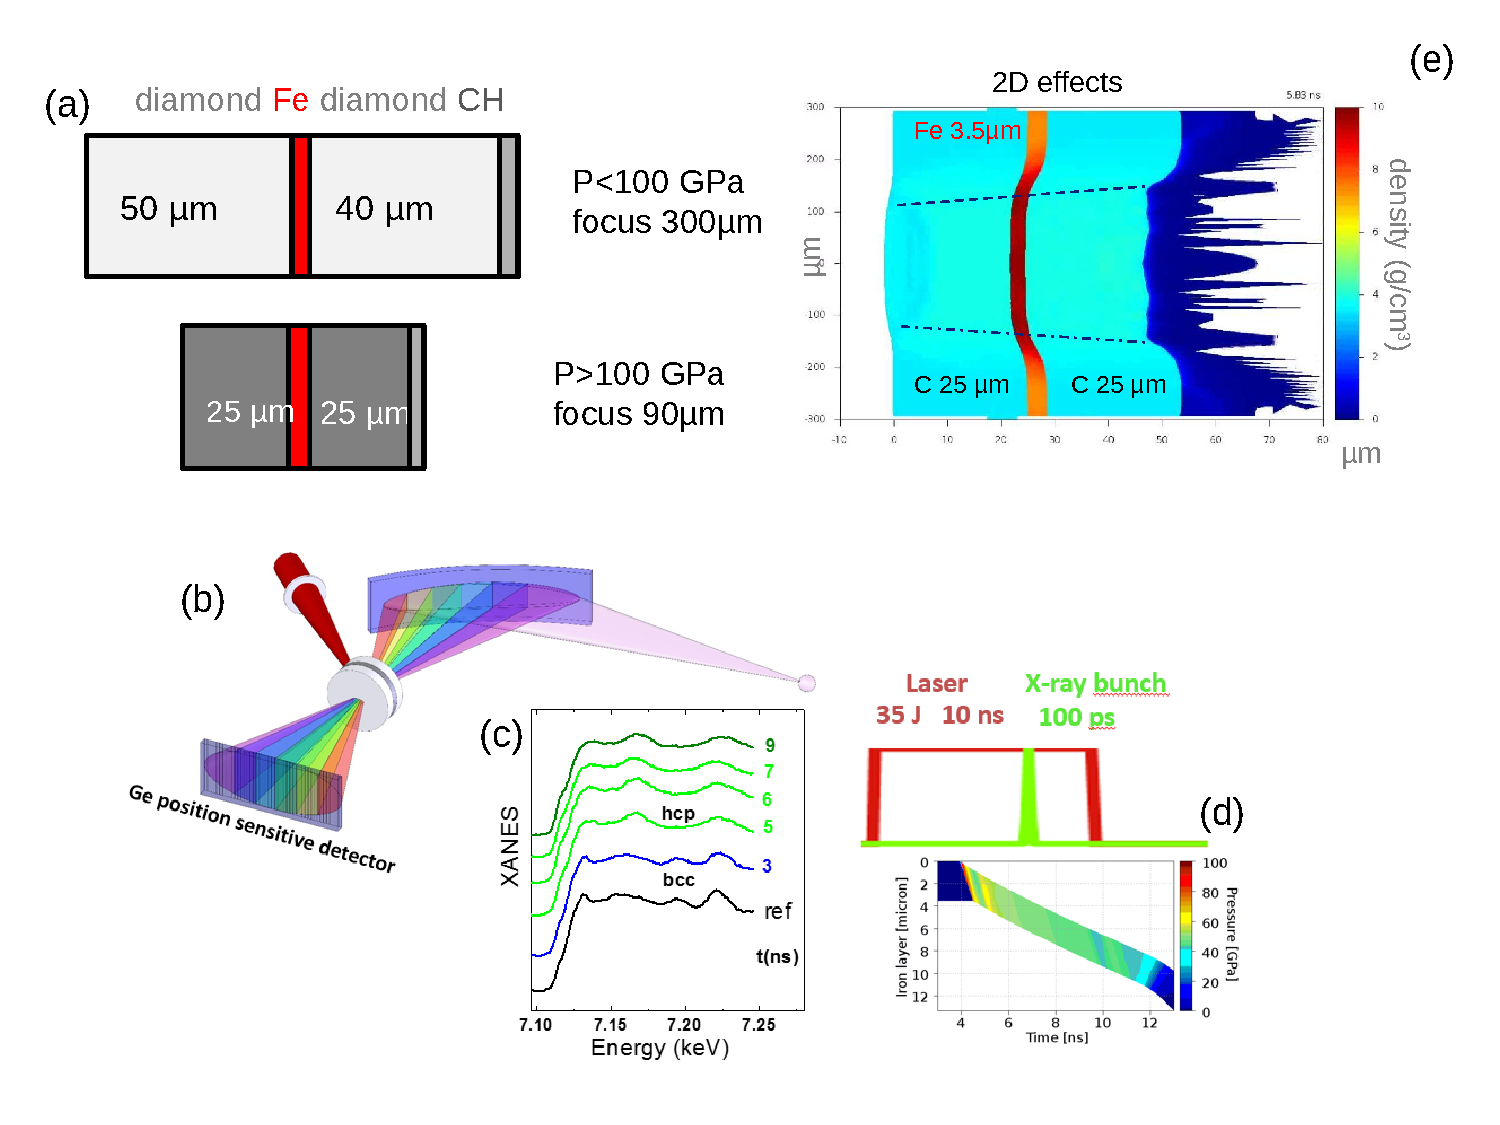
\includegraphics[width=0.8\textwidth,angle=0,clip]{torchio2016}
  \end{center}
  \caption{Target geometry (a), experimental setup (b), and XANES spectra (c)
    from ESRF ID24 experiment as reported in [Torchio et al. Scientific Reports \textbf{6}, 26402
    (2016)], 1D
  (d) and 2D (e) radiation--hydrodynamics simulation of the laser--matter
interaction.}
  \label{fig:xas_setup_rh}
\end{figure}
%
\begin{figure}[ht]
  \begin{center}
    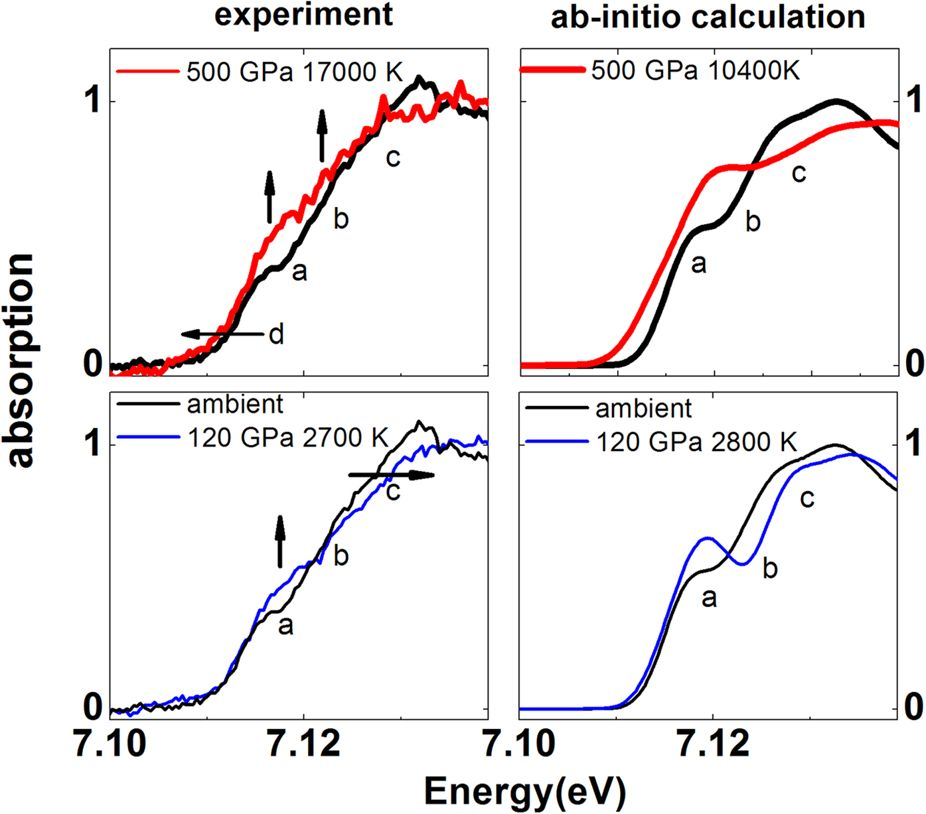
\includegraphics[width=0.8\textwidth,angle=0,clip]{xas_exp_vs_AI.jpg}
  \end{center}
  \caption{Left: Experimental EXAFS spectra close to the K--edge at two different pressure and temperature conditions realized
    in the experiment compared to ambient conditions (black line). Right: ab-initio
  molecular dynamic simulations. Labels a,b,c,d mark points in the spectrum where
  strong deviations from the ambient spectrum is observed as indicated by black
  arrows. These are
  qualitatively reproduced in the ab--initio simulations.
  Figure reproduced from [Torchio et al. Scientific Reports \textbf{6}, 26402
    (2016)] under Creative Commons Attribution 4.0 International License.}
  \label{fig:xas_exp_vs_AI}
\end{figure}
%
In Fig.~\ref{fig:xas_exp_vs_AI}, we show experimental EXAFS
spectra, measured at beamline ID24 at ESRF \cite{Torchio2016} compared to ab--initio
simulations assuming pressure and temperature conditions similar to those of
the experiment, which were modelled with RH simulations. The experimental spectra
measured at \SI{500}{\giga\pascal} pressure and \SI{1.7e4}{\kelvin} temperature
(upper left) and at \SI{120}{\giga\pascal} pressure and \SI{2.7e3}{\kelvin}
temperature (lower left), respectively, are shown in together with spectra
measured at ambient conditions (black curve). The labels a,b,c, and d mark points
in the spectrum, where the strongly compressed case shows significant
differences with respect to the ambient case. At increased pressure, a shift of
the K--edge onset to smaller energie is found, as well as a steepening of the
edge profile in the lower half of the edge retion
(\SI{<7.12}{\kilo\electronvolt}), whereas the absorption rises less steeply with respect to the
ambient case in the upper half of the edge (\SI{>7.12}{\kilo\electronvolt}).
The modelled spectra reproduce
these differences qualitatively. A more quantitative analysis and comparison
beteen theory and experiment is still outstanding.
%

We also compared 1D RH simulations for the pressure as a function
of energy on target in the case of molybdenum. Fig.~\ref{fig:rh_1d_vs_exp}
shows three measured datasets (dots) differing the the thickness of the phase plate
used to smoothen the intensity distribution over the focal spot and the pump
pulse duration. The solid lines mark the RH simulations, systematically
overestimating the pressure. This is a typical artifact of 1D RH simulations.
The systematic offset between model and data could be used to define a heuristic
correction factor to apply to 1D simulation data.
%
\begin{figure}[ht]
  \begin{center}
    \includegraphics[width=.8\textwidth,angle=0,clip]{RadHydro_Mo_1D_vs_exp}
  \end{center}
  \caption{Pressure vs. energy on target (molybdenum) for three different phase plate
  thicknesses and pulse durations. The 1D radiation--hydrodynamics simulations
  (solid lines) systematically overestimate the experimental conditions (dots).}
  \label{fig:rh_1d_vs_exp}
\end{figure}
%
\subsection{Wavefront propagation through phase gratings}
\label{sec:wpg_phasegrating}
WPG functionality has been extended to support a selection of 2D transmission gratings.
%
\begin{figure}[ht]
	\begin{center}
		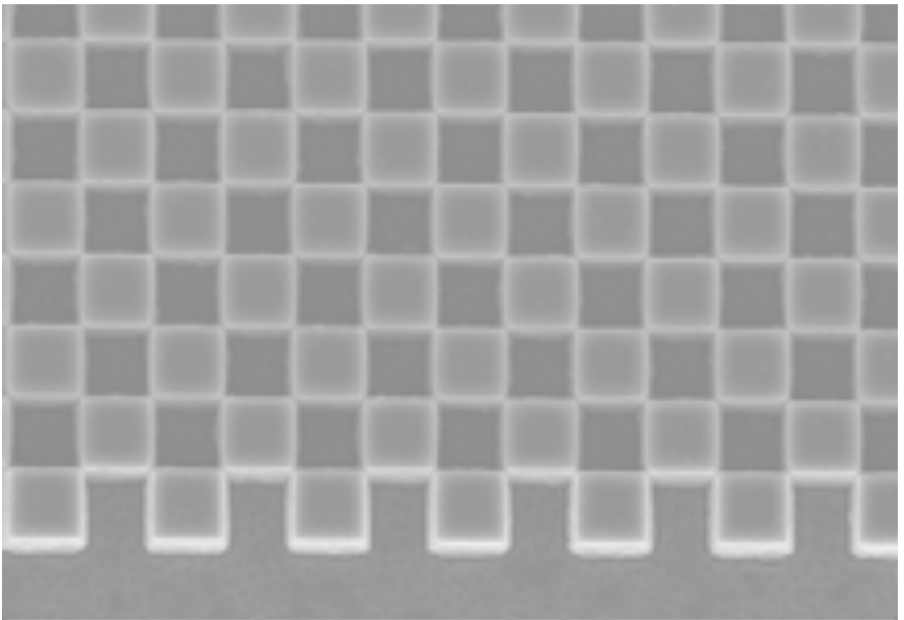
\includegraphics[width=.45\textwidth,angle=0,clip]{grating-diamond}
		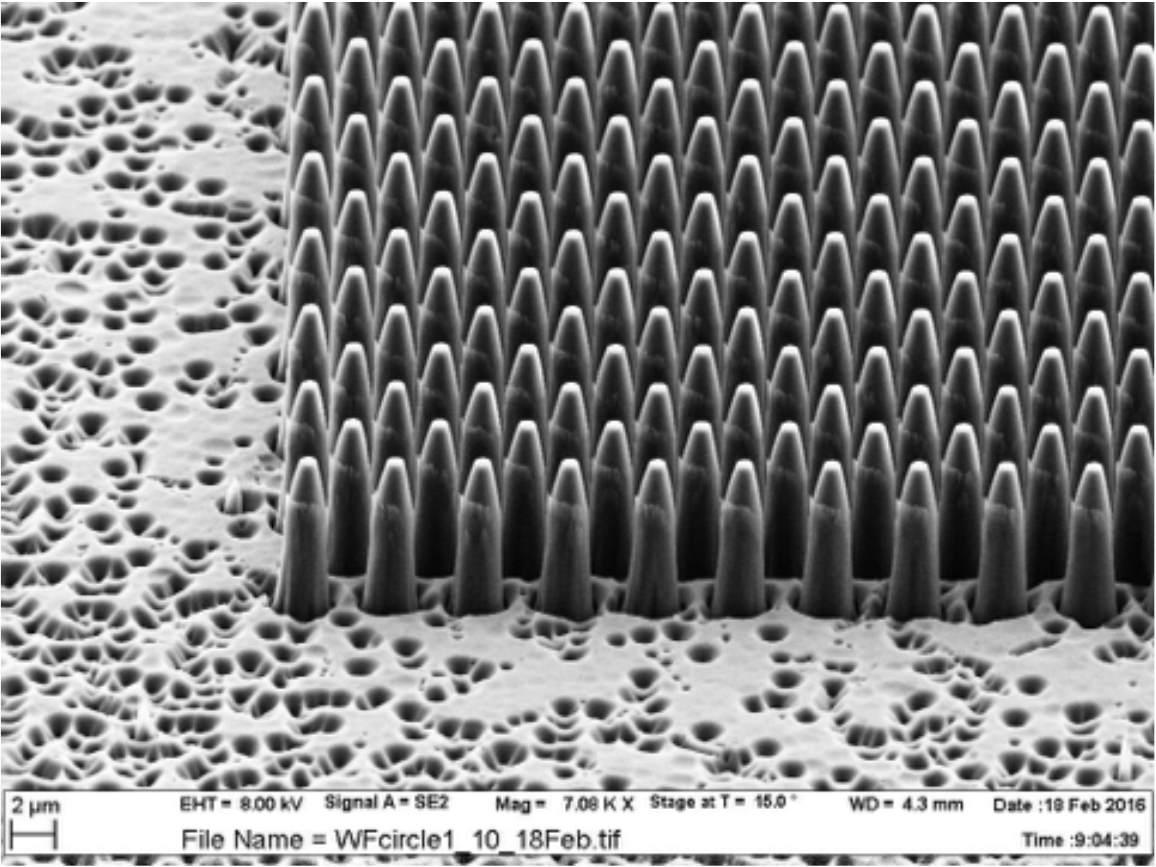
\includegraphics[width=.45\textwidth,angle=0,clip]{grating-pillar}
	\end{center}
	\caption{Checkerboard and hexagonal gratings used in conducted experiments}
	\label{fig:lm_gratings}
\end{figure}
%
The Grating element is based on the srwl class SRWLOptT (Optical Element: Transmission - generic) and its transmission properties are achieved by modifying attribute arTr - amplitude transmission and optical path difference as function of transverse position.

Grating structure can either be chosen from a predefined set (fig. \ref{fig:lm_predef}) or custom-made using a limited set of parameters.
%
\begin{figure}[ht]
	\begin{center}
		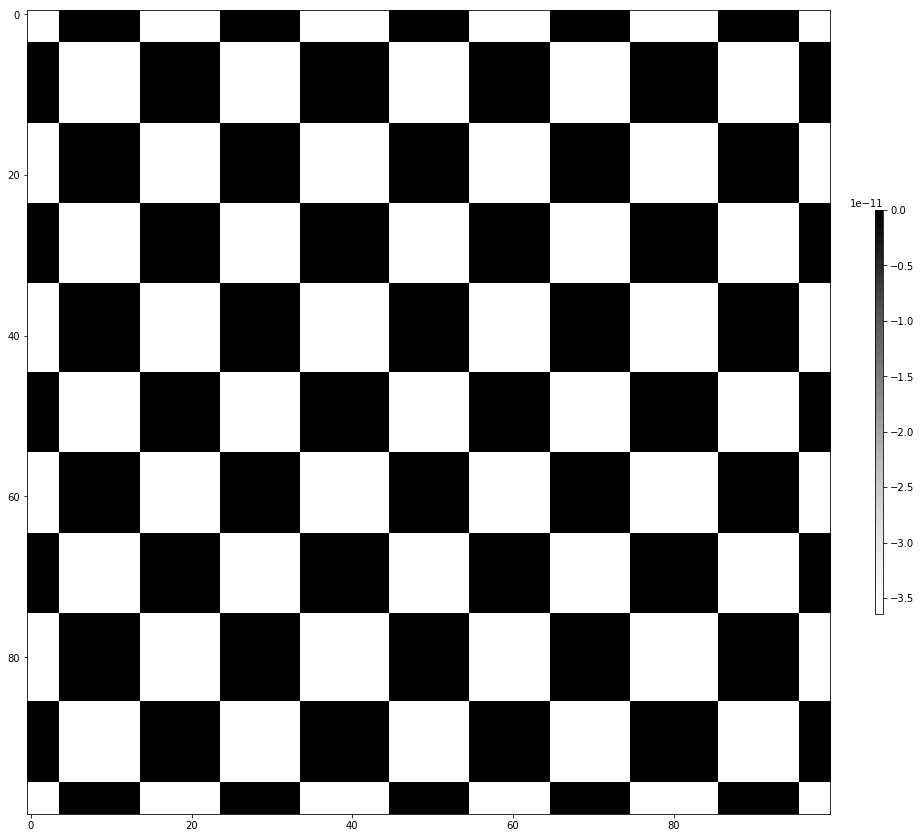
\includegraphics[width=.32\textwidth,angle=0,clip]{grating-wpg-chb}
		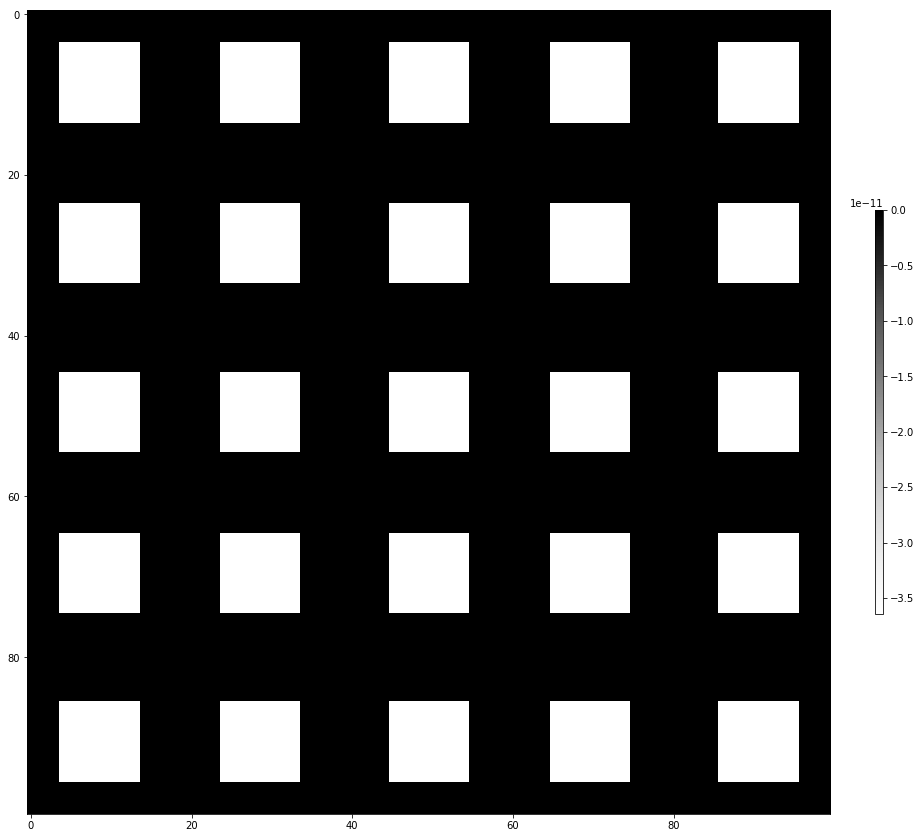
\includegraphics[width=.32\textwidth,angle=0,clip]{grating-wpg-mesh}				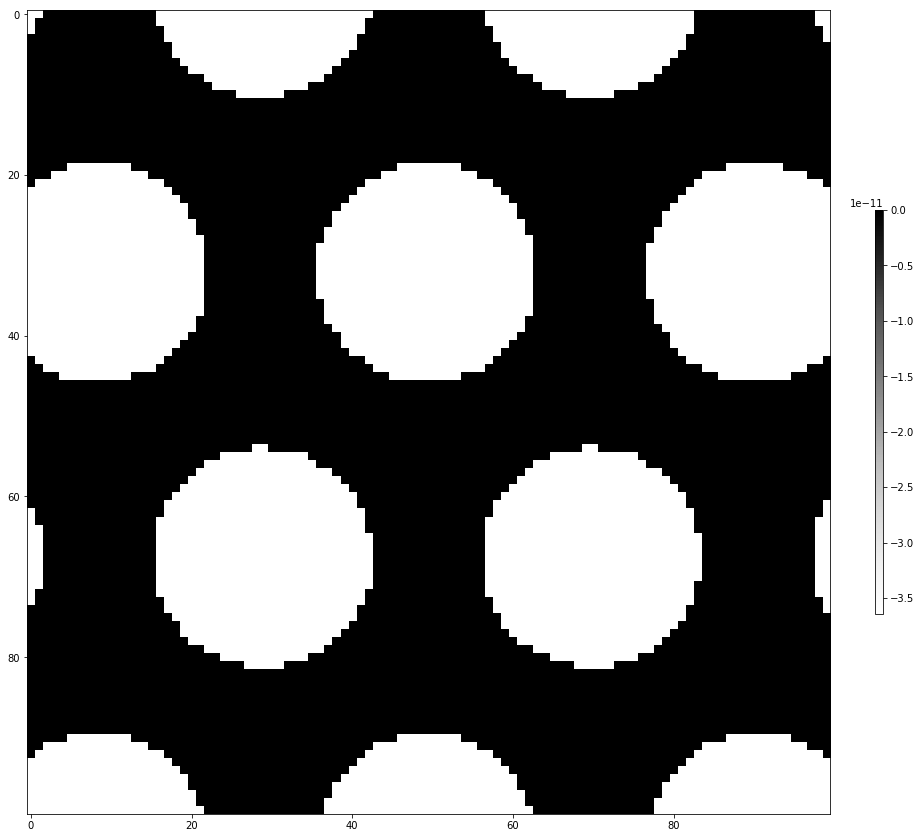
\includegraphics[width=.32\textwidth,angle=0,clip]{grating-wpg-hex}
	\end{center}
	\caption{Predefined grating structures: checkerboard, mesh and hexagonal}
	\label{fig:lm_predef}
\end{figure}
%
The predefined shapes are configured by pitch in the direction of x-axis and the y dimension can be scaled accordingly or be intentionally stretched to create rectangular structures.

The range of parameters for custom-made gratings include (fig. \ref{fig:lm_params})
%
\begin{enumerate}
	\item vectors $\vec{a}$ and $\vec{b}$ to define spacing of structural elements
	\item switch to enable halfway combinations (mesh to checkerboard)
	\item fractional parameter for $\vec{a}$ and $\vec{b}$ to specify element dimensions
	\item switch to turn element shapes into circles (hex)
	\item roll grating along the beam
\end{enumerate}
%
\begin{figure}[ht]
	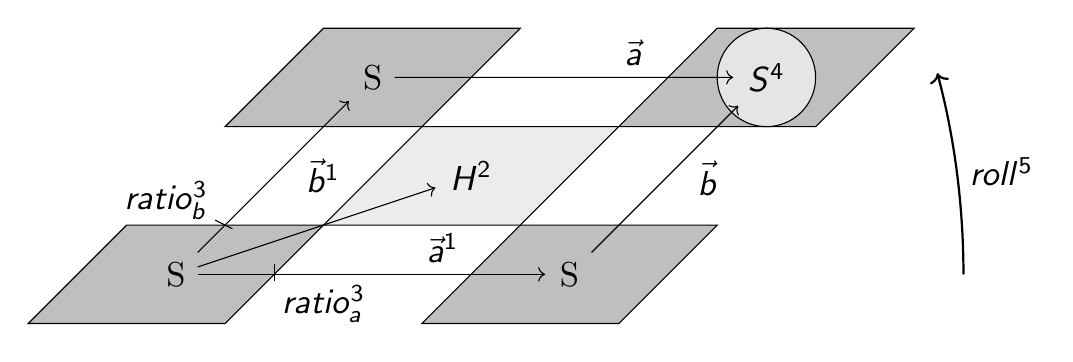
\begin{tikzpicture}[scale=1.25, every node/.style={scale=1.25},shorten >=1pt,node distance=1.0cm,on grid,auto]
%		\tikzstyle{high} = [circle, fill=gray!50]
%		\tikzstyle{mid} = [circle, fill=gray!20]
		\draw[xshift=-1.5cm,yshift=-0.5cm,fill=gray!50] (0cm,0cm) -- (2cm,0cm) -- (3cm,1cm)
		-- (1cm,1cm) -- cycle;
		\draw[xshift=2.5cm,yshift=-0.5cm,fill=gray!50] (0cm,0cm) -- (2cm,0cm) -- (3cm,1cm)
		-- (1cm,1cm) -- cycle;
		\draw[xshift=4.5cm,yshift=1.5cm,fill=gray!50] (0cm,0cm) -- (2cm,0cm) -- (3cm,1cm)
		-- (1cm,1cm) -- cycle;
		\draw[xshift=0.5cm,yshift=1.5cm,fill=gray!50] (0cm,0cm) -- (2cm,0cm) -- (3cm,1cm)
		-- (1cm,1cm) -- cycle;
		\draw[xshift=1.5cm,yshift=0.5cm,fill=gray!15] (0cm,0cm) -- (2cm,0cm) -- (3cm,1cm)
		-- (1cm,1cm) -- cycle;
		\draw[xshift=6cm,yshift=2cm,fill=gray!20] (0,0) circle(0.5);
		\node (base) at (0,0) {S};
		\node (end_a) at (4,0) {S};
		\node[coordinate] (roll) at (8,0)  {};
		\node (end_b) at (2,2) {S};
		\node (end_ab) at (6,2)  {$S^4$};
		\node (end_abh) at (3,1) {$H^2$};
		\draw[->] (base) -- (end_a) node[pos=0.7] {$\vec{a}^1$};
		\draw[->] (base) -- (end_b) node[pos=0.5,right,xshift=0.2cm] {$\vec{b}^1$};
		\draw[->] (end_a) -- (end_ab) node[pos=0.5,right,xshift=0.2cm] {$\vec{b}$};
		\draw[->] (end_b) -- (end_ab) node[pos=0.7] {$\vec{a}$};
		\draw[->] (base) -- (end_abh);% node[pos=0.7] {$\frac{\vec{a}+\vec{b}}{2}$};
		\draw[thick, ->] (roll) arc (0:15:8cm) node[midway,right] {$roll^5$};
		\draw (1,0.1) -- (1,-0.1) node[xshift=0.5cm,yshift=-0.2cm] {$ratio_a^3$};
		\draw (0.4,0.55) -- (0.6,0.45) node[xshift=-0.7cm,yshift=0.3cm] {$ratio_b^3$};
	%	\node[state,rectangle, align=center] (q_r) [] {This is a \\ square}; % Here the nodes and coordinates are defined
	%	\node[coordinate] (q_0) [right=of q_r, xshift=3cm]   {};
	%	\node[coordinate] (q_1) [left=of q_r, xshift=-3cm, yshift=1mm]   {};
	%	\node[coordinate] (q_2) [left=of q_r, xshift=-3cm, yshift=-1mm]   {};
	%	\path[->] % path and draw commands connect the nodes and coordinates to each other.
	%	(q_r) edge [] node  {This is an arrow} (q_0);
	%	\draw[->] ([yshift=-3mm]q_1) -- ([yshift=-2mm]q_r.west) node[midway,swap] {This is an arrow};
	%	\draw[->] ([yshift=3mm]q_2) -- ([yshift=2mm]q_r.west) node[midway] {This is an arrow};
	\end{tikzpicture}
	\caption{Custom grating parameters}
	\label{fig:lm_params}
\end{figure}
%
\subsubsection{Grating simulation}
We run the sample "S1 SPB CRL simplified beamline" from the WPG package(fig. \ref{fig:lm_wpg_beamline}) with a $4\mu m$ pitch, $\pi/2$ phase checkerboard grating being added $3m$ downstream of focus and wavefront measured at distances between $5.625m$ and $5.84m$ from focus with $5mm$ steps. Due to the Talbot effect from spherical wavefront, a variation in peak visibility in Fourier spectrum is to be expected in this range, which we evaluated.
At chosen "detector" range, one full period of Talbot order (even-odd-even) occurs for the diagonal pitch and two periods occur for orthogonal pitch (along x/y axis), following the equation \ref{eq:lm_talbot_order}.
%
\begin{figure}[ht]
	\begin{center}
		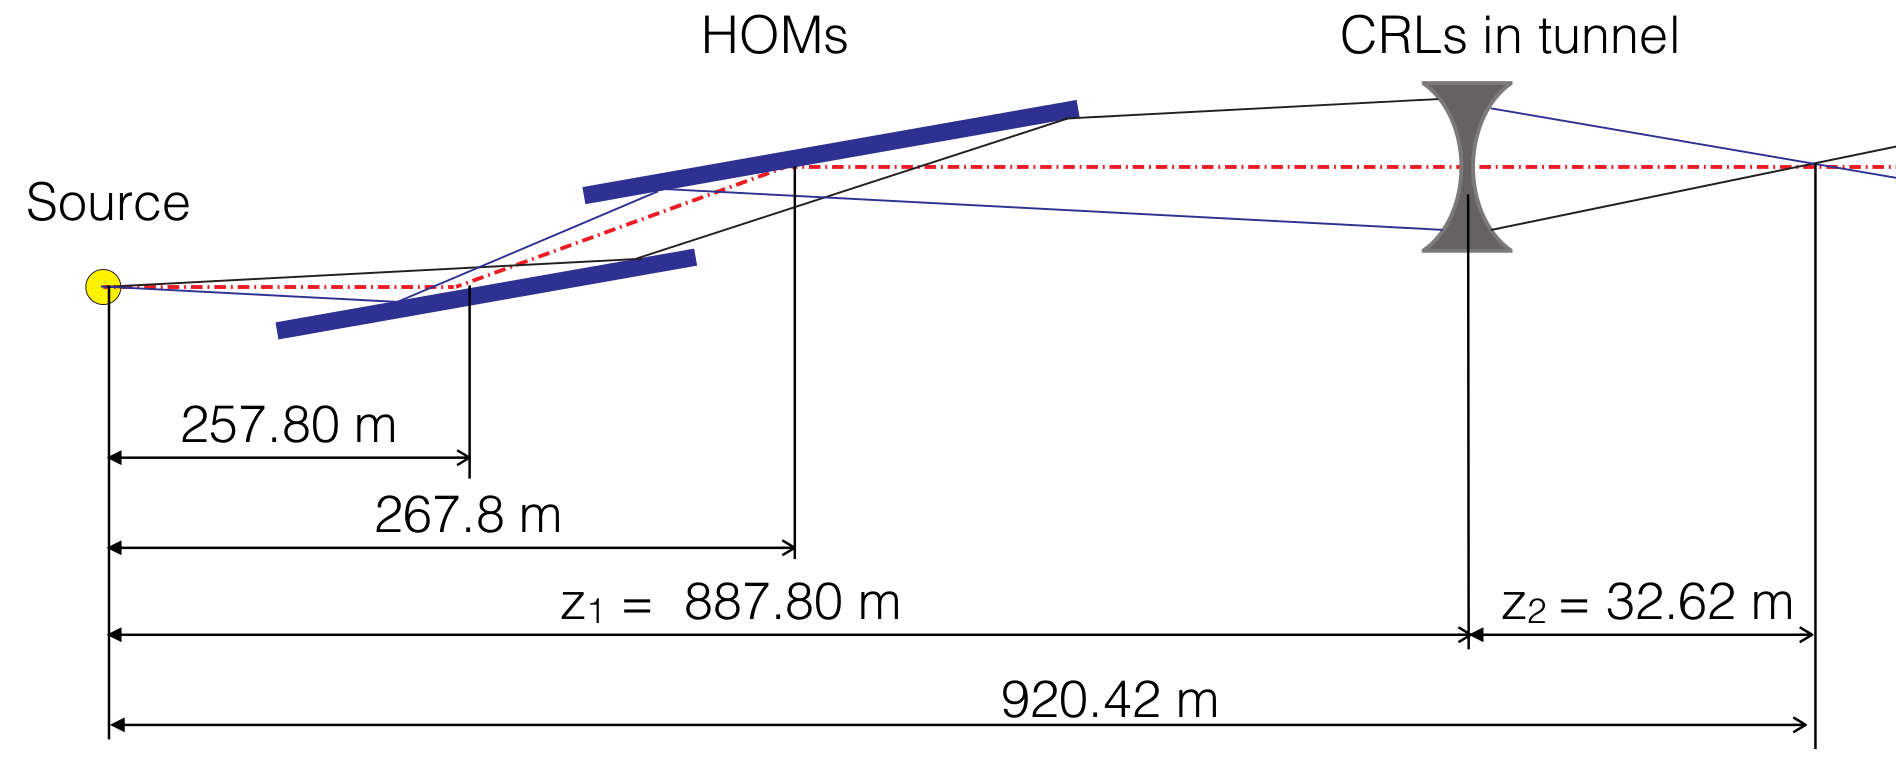
\includegraphics[width=.9\textwidth,angle=0,clip]{scheme-wpg}
	\end{center}
	\caption{Simulated simplified beamline.}
	\label{fig:lm_wpg_beamline}
\end{figure}
%
\begin{equation}
n(D) = \frac{2* \lambda * \mu ^2 * (D-G) * G}{D * pitch ^2}
\label{eq:lm_talbot_order}
\end{equation}
Where $\lambda$ is wavelength, $\mu$ specifies $\pi/2$ (1) or $\pi$ (2) phase shift, pitch is the grating pitch and D and G are distances from focus to detector and grating.

Visibility should be high for odd and low for even Talbot orders. A way to visualize it is by quantifying proximity to odd positions% (fig. \ref{fig:lm_oddness})
%
\begin{equation*}
oddness(x) = 1-(x  \mathbin{\%}  2 - 1)^2
\end{equation*}
%
The expected visibility (fig. \ref{fig:lm_visib}, left) is given by equation \ref{eq:lm_visib}. Since diagonal direction is usually dominant, orthogonal visibility is shown with factor of 0.5.
%
\begin{equation}
  visib(D) = oddness\left(n(D) \right)
  \label{eq:lm_visib}
\end{equation}
%
Values calculated from the simulated beamline (fig. \ref{fig:lm_visib}, right) closely resemble the expected pattern and agree with other results we got from actual experiments.
We observed a slight jitter not only in simulation visibility values, but also directly in wavefront calculated intensity. All the simulations were run with parameter $num\_points$ set to $1000$ and the grating defined at $2000$ data points (20 per orthogonal pitch). More precise results could be expected at higher resolutions at the cost of increased computation times.
%
\begin{figure}[ht]
	\begin{center}
		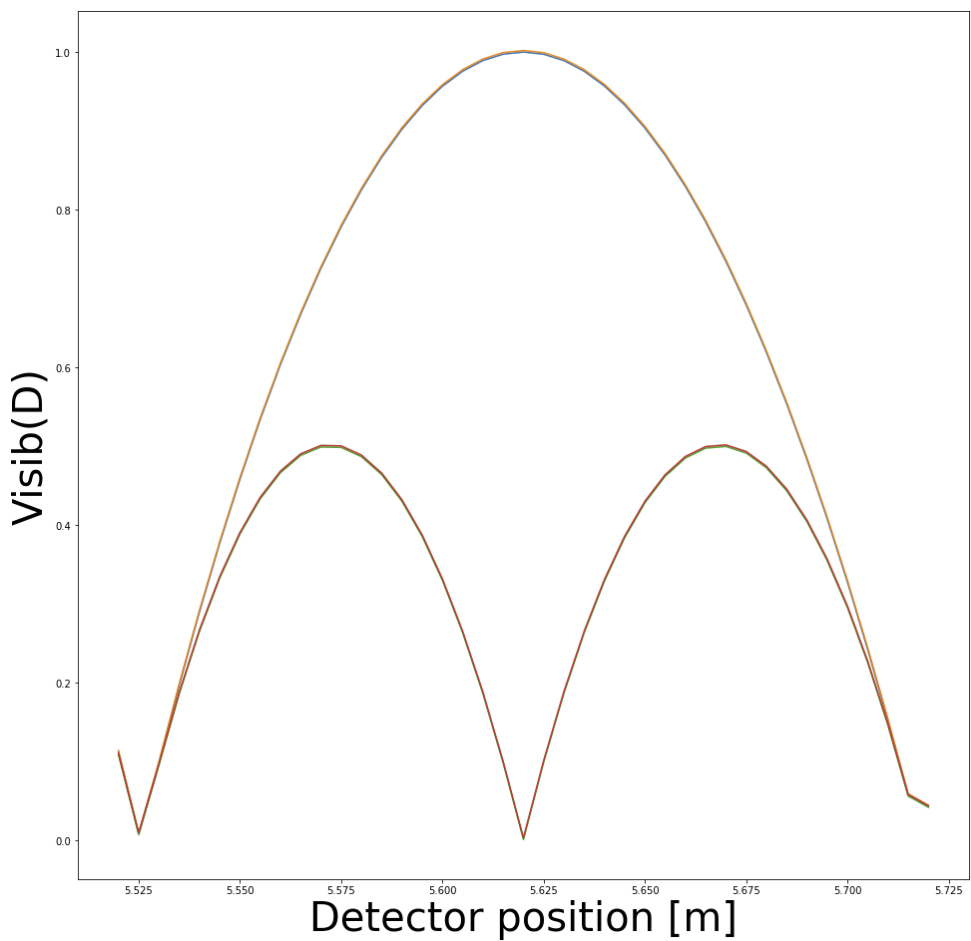
\includegraphics[width=.45\textwidth,angle=0,clip]{plot-talbot-visibility}
		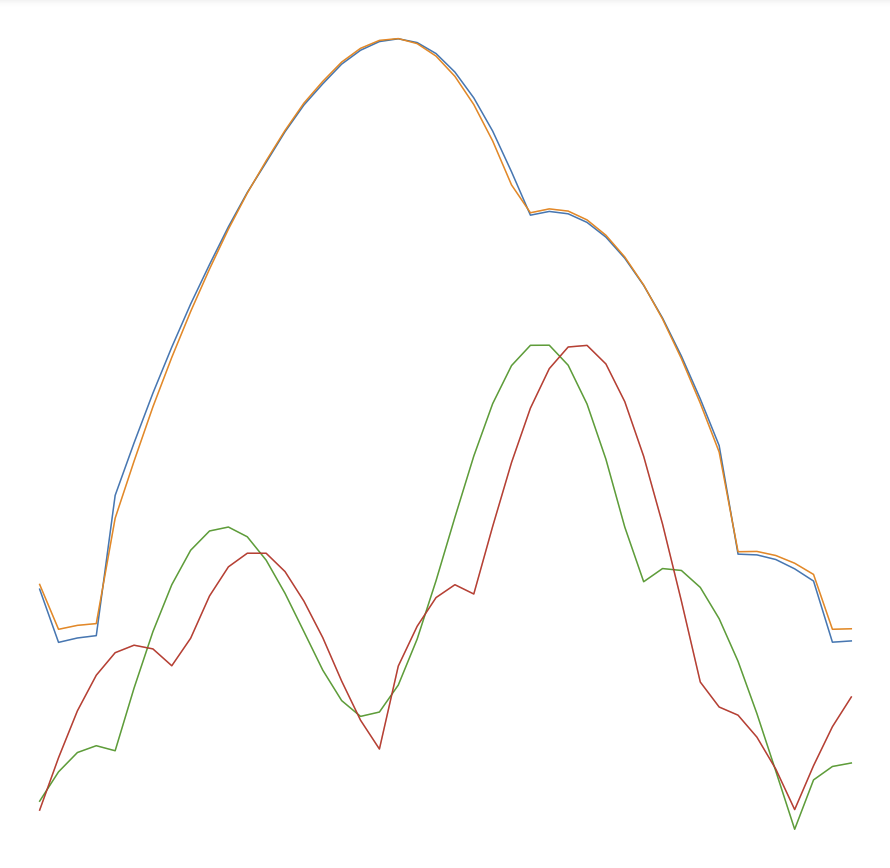
\includegraphics[width=.45\textwidth,angle=0,clip]{plot-wpg-visibility}
	\end{center}
	\caption{Visibility: expected and simulated. Diagonals: orange/blue; x/y: green/red}
	\label{fig:lm_visib}
\end{figure}
%
\FloatBarrier
%
\section{High Performance Computing Benchmarks}
\subsection{Single--particle imaging simulation pipeline}
The single--particle imaging simulatoin pipeline consists of
%
\begin{enumerate}
  \item pulse propagation
  \item photon--matter interaction
  \item diffraction
  \item detector response (optional)
\end{enumerate}
%
Each of these modules have very different and demanding computational resource
requirements. We present benchmarking results for few selected modules which
represent performance bottlenecks in the simulation pipeline.
%
\subsubsection{Wavefront propagation}
The wavefront propagation utilizes the software Synchrotron Radiation Workshop
(SRW), a legacy C library with historically very limited options for
parallelization. Recently, there have been three major developments:
\begin{enumerate}
  \item Insertion of openMP macros to enable shared--memory parallelism
  \item Multicore parallel execution of propagation of multiple FEL source
    pulses.
  \item MPI parallel calculation of independent coherent modes for partially
    coherent wavefront propagation.
\end{enumerate}
%
1) and 2) have been realized in SIMEX, 3) is an independent development in the radiation source
simulation and propagation framework SiRepo
\url{www.github.com/radiasoft/sirepo}. Fig.~\ref{fig:srw_speedup} shows the
speedup of a single SRW wavefront propagation resulting from the insertion of
openMP pragmas in the SRW source code.
%
\begin{figure}[ht]
  \begin{center}
    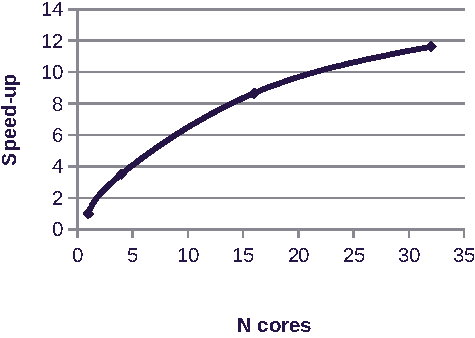
\includegraphics[width=0.8\textwidth,angle=0,clip]{srw_speedup-crop}
  \end{center}
  \caption{Speedup of WPG/SRW wavefront propagation for a single source input
  file using openMP shared--memory parallelism.}
  \label{fig:srw_speedup}
\end{figure}
%
\begin{table}
  \centering
  \begin{tabular}{rrrr}
    \textbf{Threads x MPI processes} & \textbf{Number of nodes} &
    \textbf{Wall time (min)} & \textbf{Time/input file (s)} \\
    \hline
    1x1        & 1     & 660       &  1031 \\
    40x1       & 1     &  65       &    98 \\
    4x10       & 4     &   7.5     &    45 \\
    8x5        & 8     &   4.2     &    51 \\
  \end{tabular}
  \caption{Total wall time taken by the propagation of 40 individual source files with hybrid
  openMP/MPI parallelism in SRW. Note how the distribution of MPI processes over nodes
and threads influences the walltime and the time to process each file.}
  \label{tab:srw_hybrid_timings}
\end{table}
%
\subsubsection{Radiation damage}
The radiation damage module is by far the most compute intensive part of the SPI
pipeline, determining $\approx 90\%$ of the total wall time\footnote{The wall
  time defines the time elapsed between the start and the end of a computer
  program run.} of one
start--to--end propagation. The code \textit{xmdyn and xatom}, provided by
CFEL, DESY \cite{Jurek2016} utilizes GPGPU cards. MPI or shared memory
parallelism are currently not implemented, only one GPGPU card can
be utilized at a time. Our benchmarks therefore compare the performance on
different GPGPU variants. The test case is a trajectory of the 2NIP protein
irradiated by a \SI{10}{\femto\second} (FWHM) pulse of
\SI{5}{\kilo\electronvolt} FEL photons (pulse energy \SI{\approx 1}{\milli\joule}).
%
\begin{table}
  \centering
  \begin{tabular}{rrr}
    \textbf{GPU model} & \textbf{Total wall time first run (s)} & \textbf{Total
    wall time subseq. run (s)}\\
    \hline
    K20X  & 580 & 568 \\
    K40X  & 484 & 470 \\
    P100  & 470 & 466 \\
  \end{tabular}
  \caption{Wall time for a single \textit{xmdyn and xatom} run on different
NVIDIA(C) GPGPU cards.
The first run takes longer because the atomic transition database
has to be populated.}
  \label{tab:xmdyn_performance_nvidia}
\end{table}
%
\subsubsection{Diffraction}
%
Diffraction calculations are performed with the code \textit{pysingfel}. To
enhance performance, this code uses the \textit{numba} library to facilitate
just--in--time compilation for available hardware of compute intensive parts.

Typically, one simulation run produces many
diffraction patterns. Since all pattern calculations are independent, the
best speedup can be obtained by parallelizing the diffraction simulation over the
number of diffraction patterns requested. Fig.~\ref{fig:pysingfel_performance}
shows the speedup by comparing the Wall times for computation of
100 patterns on a shared memory system with 1, 10, and 100 MPI processes,
respectively.
\begin{figure}[ht]
  \begin{center}
    \begin{tikzpicture}
      \begin{loglogaxis}[
        title=Pysingfel performance,
        xlabel={Number of MPI processes},
        ylabel={Speedup}
      ]
      \addplot[blue,mark=*] table {pysingfel_timings.dat};
      \addplot[domain=1:100] {x};
      \end{loglogaxis}
    \end{tikzpicture}
  \end{center}
  \caption{Speed up factor for parallel computation of 100 diffraction patterns with
    \textit{pysingfel} using MPI parallelization. (the black line represents linear scaling).}
  \label{fig:pysingfel_performance}
\end{figure}
The case with 100 MPI ran on 2 separate nodes, whereas the cases with 1 and 10 processes
ran on a single node with shared memory. The additional data communication
between the nodes results in a reduced speedup between 10 and 100 nodes
as compared to the speedup between 1 and 10 nodes. Also, the serial portion of
the code (parsing the sample file, geometry calculations) result in a
sub--linear  speedup.

\subsection{High--power laser--matter interaction (\textit{picongpu})}
Performance benchmarks for the particle--in--cell code \textit{picongpu} for the
simulation of high--power laser--matter interaction are presented in
\cite{Bussmann2013}, see also Ref.~\cite{Zenker2016} for an updated version. We
show in Fig.~\ref{fig:picongpu_strongscaling} the speedup (strong scaling)
achieved by increasing the number of GPUs between 2 and 1024
demonstrating the near--linear scaling. More performance
analysis data is presented in Ref.~\cite{Bussmann2013} including scalings up to
18432 GPUs and also weak scalings.
\begin{figure}[ht]
  \begin{center}
    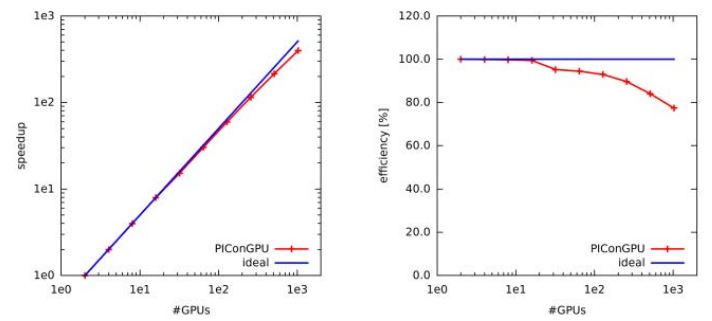
\includegraphics[width=0.8\textwidth,angle=0,clip]{figures/picongpu_strongscaling}
  \end{center}
  \caption{Speedup (left) and efficiency (right) from strong scaling performance
    analysis between 2 and 1024 GPUs for the PIC code
    \textit{picongpu}. Reproduced from [Bussmann et al. ``Radiative signatures
    of the relativistic Kelvin-Helmholtz instability'', Proc. SC'13 (2013)].}
  \label{fig:picongpu_strongscaling}
\end{figure}
%
\FloatBarrier
\section{SIMEX as a Service}
\subsection{Introduction}
For the task 4.3.2 \textit{Provide a framework towards a service to users [\dots\ ] } we set up an instance of \textit{JupyterHub} for the users of the \textit{Maxwell Cluster} at \textsc{DESY}.
Users of the \textit{SIMEX} code are familiar with the computing environment at \textsc{DESY} and use the cluster in many ways.
To run heavy computations on the cluster users have to submit a job to \textit{SLURM} which will then allocate ressources to the users' jobs and run them.
This is a well-established workflow for simulations and data reduction pipelines where the result of the
computation can be delayed by days from the time of submission.
For other use-cases though, users need near to instantaneous feedback from their input.
This is what \textit{iPython} does. It is a interactive python shell that evaluates commands - or multi line command blocks - one by one and returns a result directly.
The iPython notebook was a web-based frontend to iPython that was then renamed into the Jupyter Notebook after other backends became popular.
Doing work with the Jupyter Notebook on a remote server or a High Performance Cluster requires a few steps, setting up an SSH Tunnel with port forwarding, logging onto the server and then starting the notebook manually.
If a user wants more advanced features like password protection
The JupyterHub is a development that is meant for environments where many users need to access a Jupyter Notebook and all those steps are done automatically and users only need to log in with their username and password.

We developed example notebooks which can be used as a starting point by
\textit{simex} users to learn the workflow and to run their own simulations by
modifying the example. We document in appendix \ref{appendix:notebooks}
two example workflows for simulation of
single--particle imaging and for nanocrystalography. Both notebooks can be
obtained from the EUCALL software repository.
\url{https://www.github.com/eucall-software/simex_notebooks}.

\subsection{Features of the JupyterHub at DESY}
The JupyterHub we set up uses a lot of infrastructure already available at DESY. In the following we explain how they were included into an instance to make data analysis more convenient.
Features of the \textit{JupyterHub} Instance include:

\begin{itemize}
 \item Encryption via SSL using an DFN (Deutsches Forschungsnetzwerk) inheritance certificate to provide user data security
 \item Integration into the existing LDAP authentication at DESY
 \item Connection to the SLURM ressource manager on the Maxwell Cluster
 \item Customization of the Notebook Spawner to provide access to the GPFS file system
 \item Addition of Various Python Kernel Versions and other demanded languages such as R \& bash kernels
 \item Using the Maxwell Cluster as an infrastructure to provide computing power
\end{itemize}
%
\subsection{Using the JupyterHub and SimEx}
To use the JupyterHub at DESY one has to visit the website
\url{https://max-jhub.desy.de} while on the DESY-XFEL Network.
Opening the ports to the Internet is work in progress and needs the server to be isolated in the demilitarized zone (DMZ) which is a different network section and has special firewall rules.
Users then see the scrren shown in fig.~\ref{fig:jhub_start} which has been customized to show the DESY Logo and shows the \textit{Secure} Website lock so User know their data is protected.
Users then have to enter their DESY credentials which are passed to the LDAP server to check if the password is correct.
%
\begin{figure}
  \centering
  \begin{subfigure}{0.45\textwidth} % width of left subfigure
	  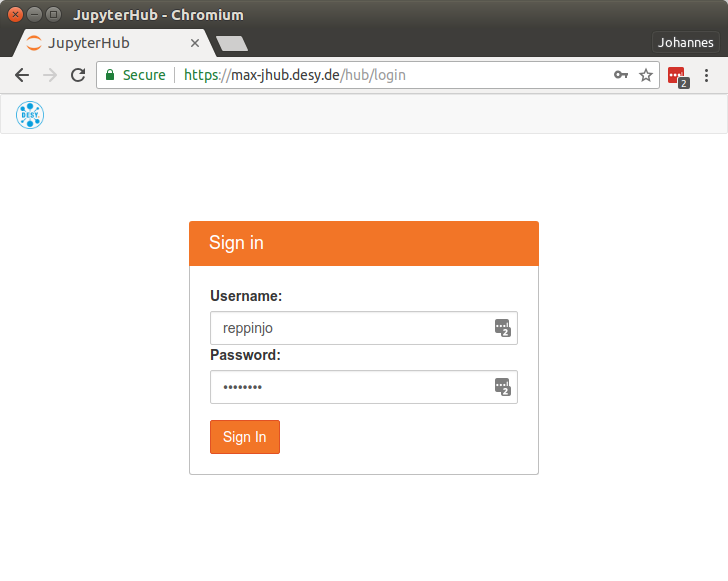
\includegraphics[width=\textwidth]{figures/jhub001.png}
	  \caption{View of the login Page of the JupyterHub instance witht the url
        \url{https://max-jhub.desy.de}} % subcaption
  \end{subfigure}
  \vspace{1em} % here you can insert horizontal or vertical space
  \begin{subfigure}{0.45\textwidth} % width of right subfigure
	  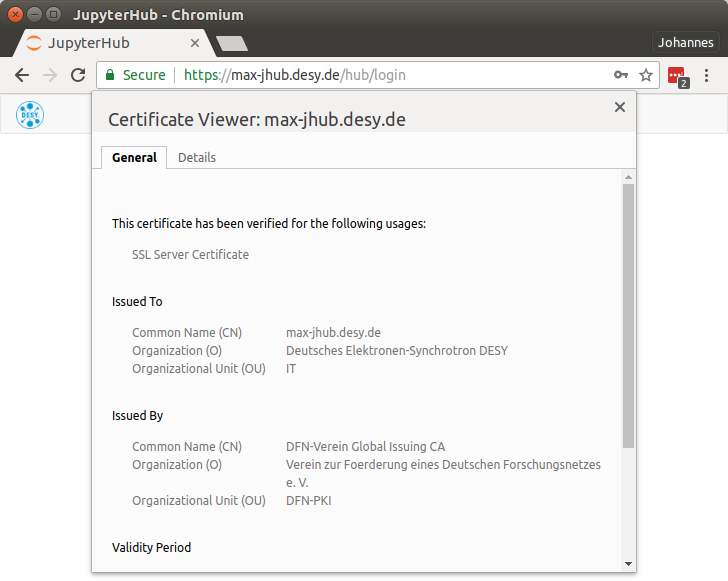
\includegraphics[width=\textwidth]{figures/jhub002.png}
	  \caption{The website has a trusted SSL certificate so users can trust our website.} % subcaption
  \end{subfigure}
  \caption{Screenshots of the JupyterHub login page and its SSL certificate}
  \label{fig:jhub_start}
\end{figure}

After login on, users are presented with a choice, shown in
fig.~\ref{fig:jhub_spawn}, where their notebook should run. There is a shared
partition where users can
%
\begin{figure}
  \centering
    \begin{subfigure}{0.45\textwidth} % width of left subfigure
	  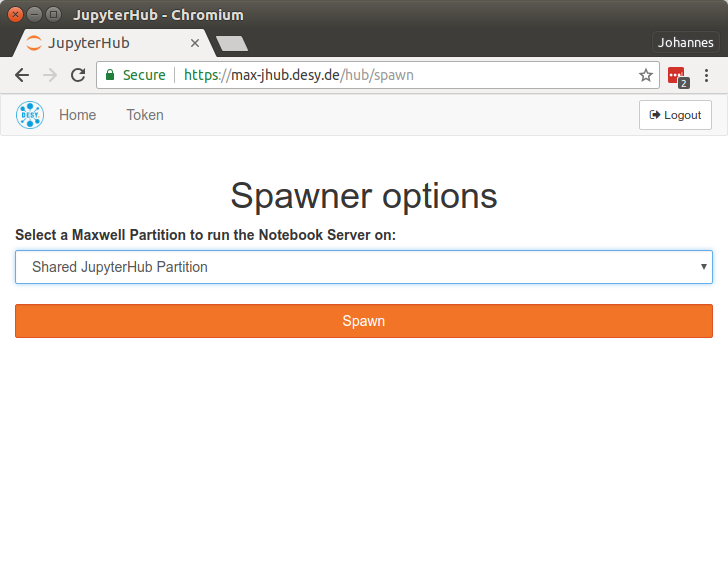
\includegraphics[width=\textwidth]{figures/jhub004.png}
	  \caption{Before getting to the Notebook, users see the choice of spawner options for the partition to run the notebook on.} % subcaption
  \end{subfigure}
  \vspace{1em} % here you can insert horizontal or vertical space
  \begin{subfigure}{0.45\textwidth} % width of right subfigure
	  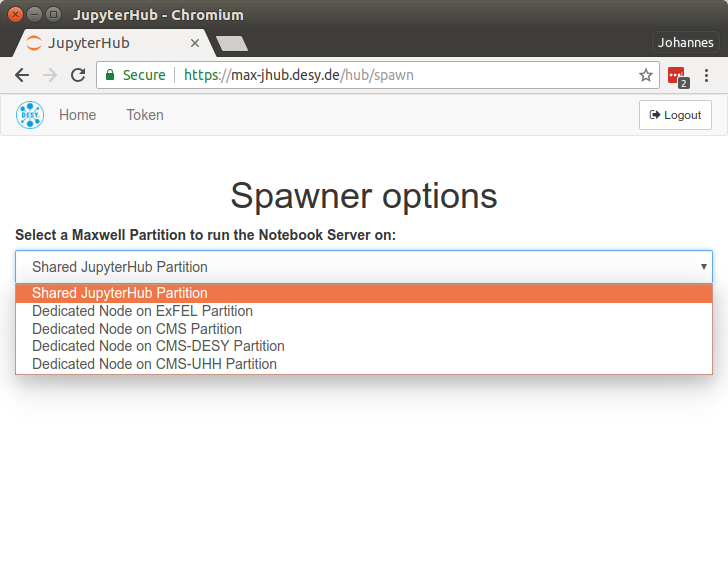
\includegraphics[width=\textwidth]{figures/jhub005.png}
	  \caption{A shared Jhub partition and workgroup partitions for more heavy load usage are available, the shared one is the default.} % subcaption
  \end{subfigure}
  \caption{After the login using the DESY credentials was successful, the user has multiple options to select from for the spawner to start the notebook server}
  \label{fig:jhub_spawn}
\end{figure}
%
Once the user has selected the partition a SLUM job is submitted that starts the Notebook Server and a connection is established and users see the screen depicted in fig.~\ref{fig:jhub_work}. On the right panel the options to start are shown. This is neccessary so users have access to their group specific partition if they want to do interactive computations with a full node and not just sharing ressources.
%
\begin{figure}
  \centering
    \begin{subfigure}{0.45\textwidth} % width of left subfigure
	  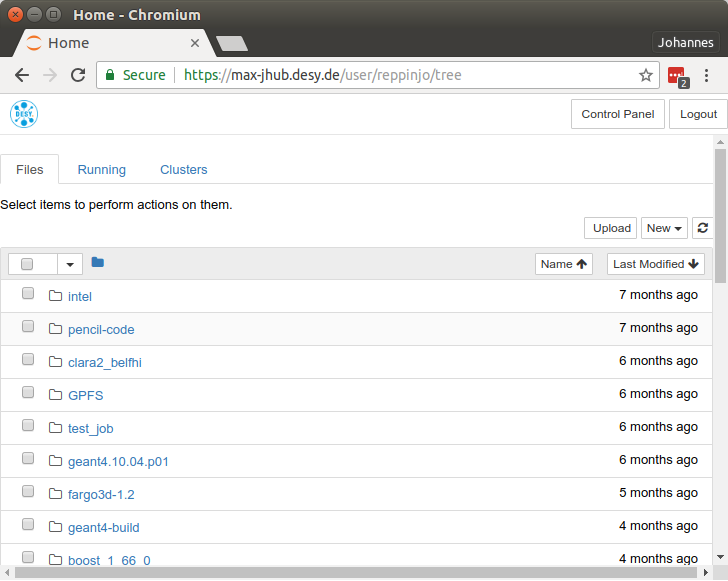
\includegraphics[width=\textwidth]{figures/jhub006.png}
	  \caption{This is a the screen users see when the notebook is launched. The files and folders correspond to the users' home directorys.} % subcaption
  \end{subfigure}
  \vspace{1em} % here you can insert horizontal or vertical space
  \begin{subfigure}{0.45\textwidth} % width of right subfigure
	  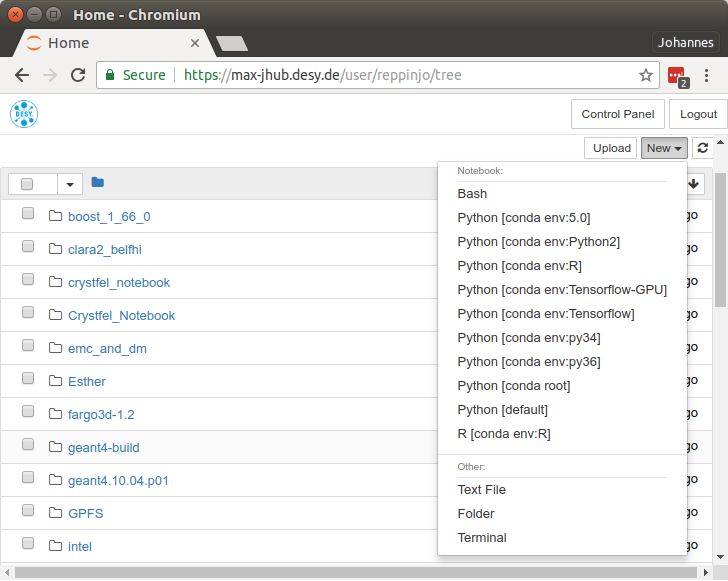
\includegraphics[width=\textwidth]{figures/jhub007.png}
	  \caption{When choosing a new kernel users have many options of Python versions, R \& a bash kernel, text files editing and a terminal session.} % subcaption
  \end{subfigure}
  \caption{Screenshots of the JupyterHub Instance at DESY, at different stages of the workflow. The images on the top show the login page and the SSL certificate, the middle the Spawner options and the bottom two screenshots show the User's files and folder as well as the available Kernels that can be used to start a Notebook}
  \label{fig:jhub_work}
\end{figure}
%
Once the server is started and and a notebook is openend, users of the \textit{SimEx} code can execute code cells
to import the module and functions they use in their regular python-driven workflow they are used to without the Jupyter Notebook, as is shown in fig.~\ref{fig:simex_import}.
The advantage is now that plots can be displayed inline, so no X-forwarding is needed.
Also, the Jupyter Notebook supports cells with \textit{Markdown} format, so documenting the work and coding progress
can be done by adding cells with headings, text and even \LaTeX style text blocks.
%
\begin{figure}
 \centering
 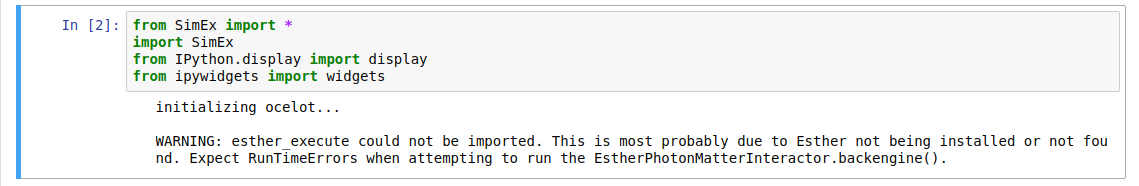
\includegraphics[width=0.9\textwidth]{figures/simex_import_jhub.png}
 \caption{The Jupyter Notebook executes code in \textit{cell blocks} that can be executed individually. The import statement to make the \textit{SimEx} modules available runs and user sees immediately if it fails or the import was successful}
 \label{fig:simex_import}
\end{figure}
%
\FloatBarrier
%%%%%%%%%%%%%%%%%%%%%%%%%%%
\printbibliography[title={References}]
%
%\printbibliography[keyword=submitted, title={Submitted articles}]
%
%\printbibliography[keyword=inpreparation, title={Articles in preparation}]
%
%\printbibliography[keyword=eucall, keyword=report, title={Project reports}]
%
%%%%%%%%%%%%%%%%%%%%%%%%%%%
\FloatBarrier
\appendix
\section{Example workflows}
\label{appendix:notebooks}
\subsection{Start--to--end single particle imaging}
\includepdf[pages=-]{contributions/XFEL/demos/s2e_spi/start_to_end_demo.pdf}
%
\subsection{Nanocrystal diffraction}
\includepdf[pages=-]{contributions/XFEL/demos/xstal/xstal_diffraction.pdf}
%
%%%%%%%%%%%%%%%%%%%%%%%%%%%
\end{document}
%%%%%%%%%%%%%%%%%%%%%%%%%%%
